\subsection{Google Chrome Developer Tools}
Google Chrome Developer Tools (\path{https://www.google.de/intl/en/chrome/browser/}) is an integrated toolkit contained within Googe Chrome.\\
I allows to view the Requests and Responses (and their headers) that are done while a website is browsed. Additionally it supports to export a Request as curl command that can be used in the terminal and resembels an exact copy of the first Request.\\
The Developer Tools further allow to inspect and edit cookie data.\\
One of the main functionality is the possibility to view and edit the DOM and CSS rules as well as directly executing JavaScript on the website.
\begin{figure}[ht]
	\centering
	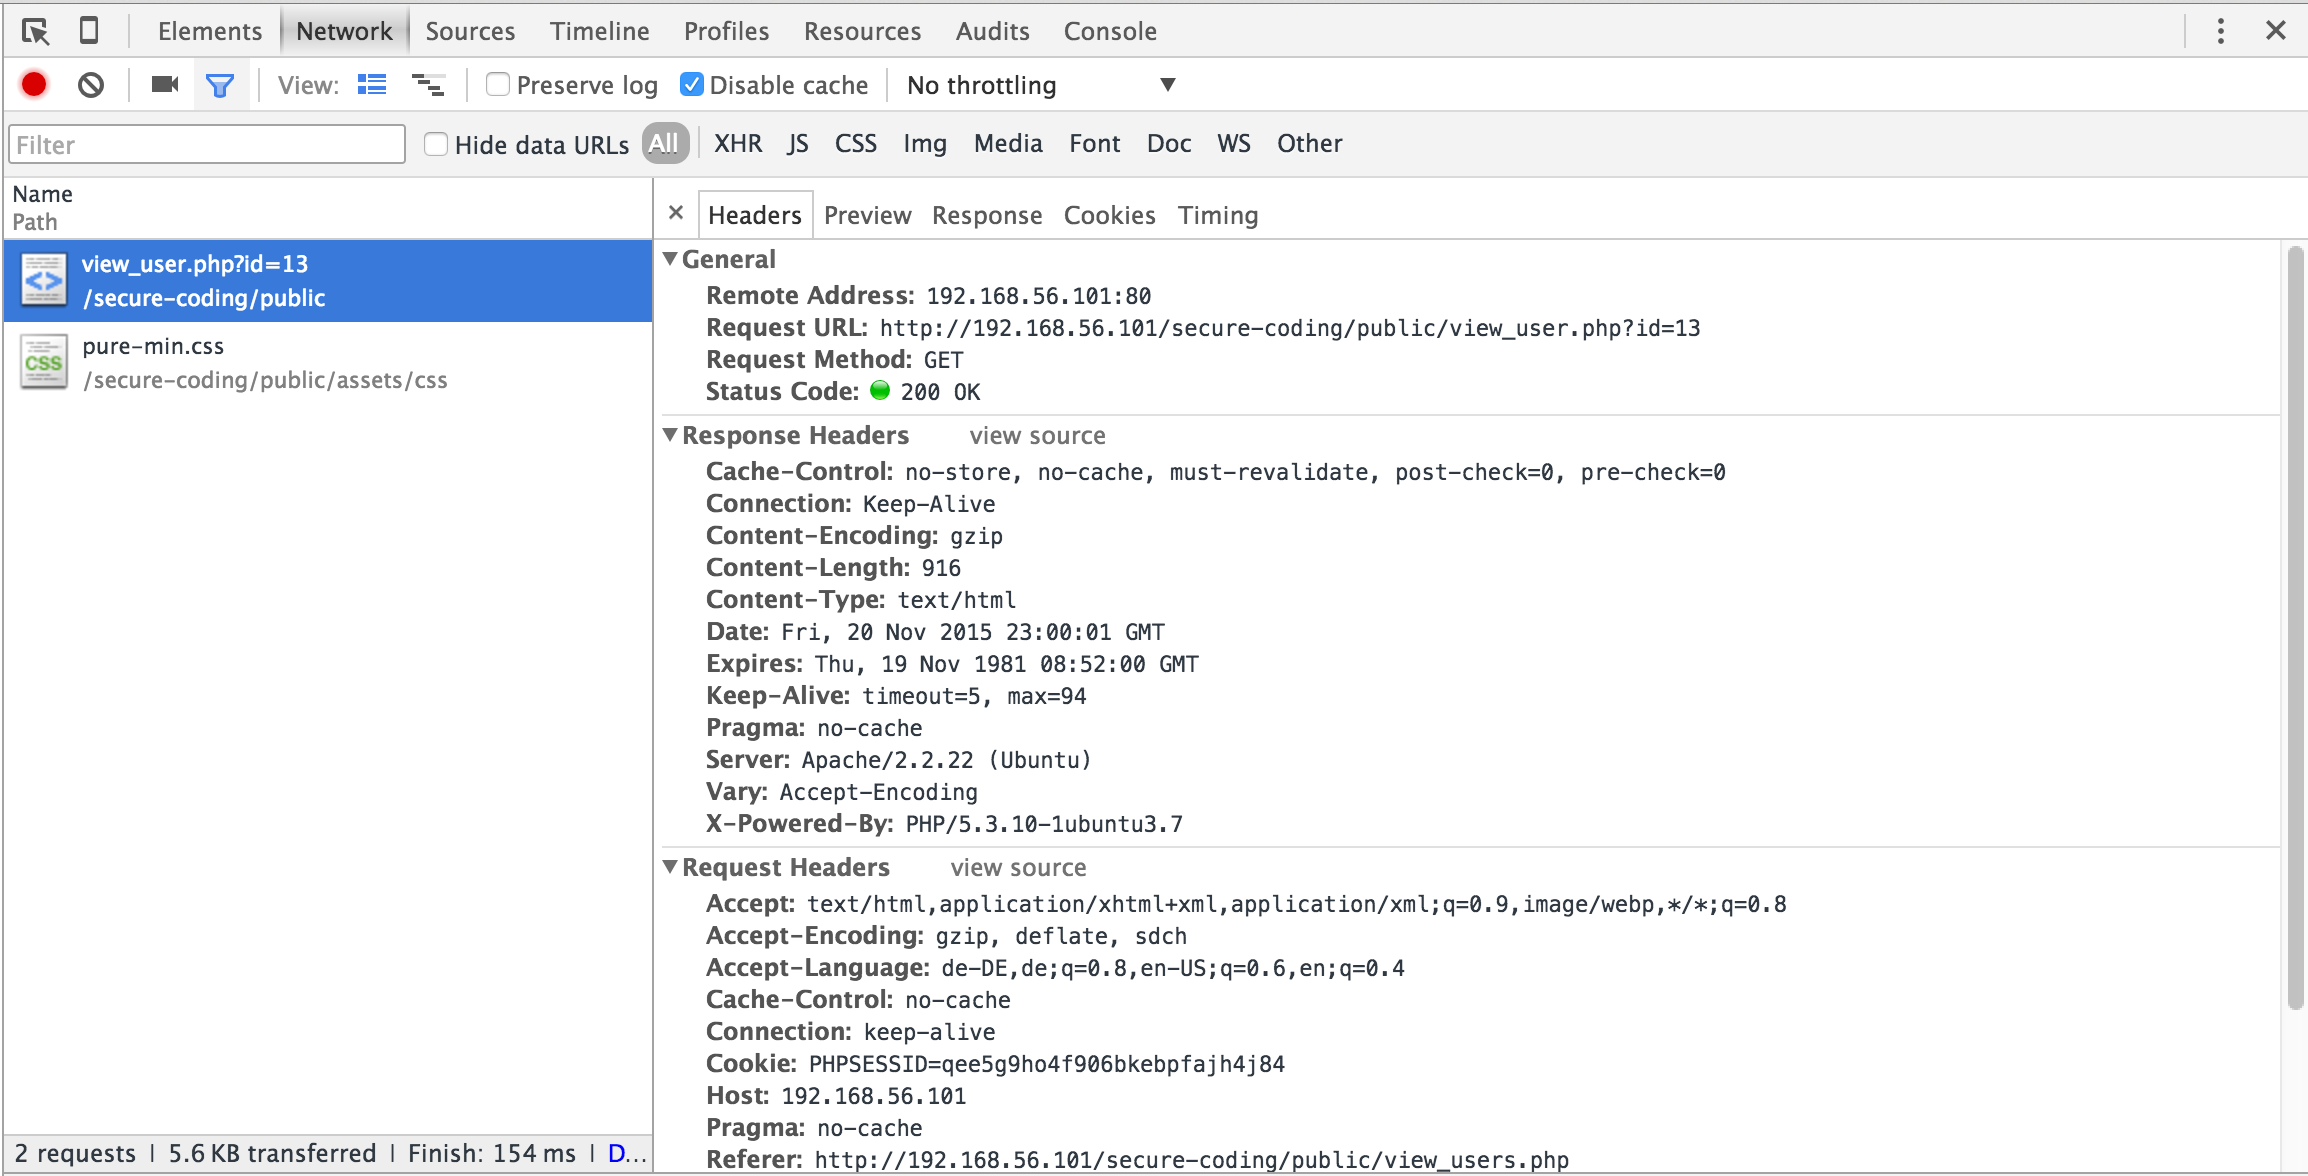
\includegraphics[width=.8\linewidth]{figures/tool_chrome_dev_tools.png}
	\caption{Google Chrome Developer Tools Network Analysis}
	\label{fig:tool_chrome_dev_tools}
\end{figure}
